\documentclass[10pt, letterpaper]{article}
\usepackage[cm]{fullpage}
\usepackage{algpseudocode}
\usepackage{algorithm}
\usepackage{graphicx}
\usepackage[section]{placeins}
\usepackage[table]{xcolor}
\usepackage{amsmath}
\usepackage[margin=0.7in]{geometry}

\algrenewcommand\Return{\State \algorithmicreturn{} }%

\title{0-1 Knapsack}
\author{Daiwei Chen \and Joseph Watts}

\begin{document}
\maketitle
	\begin{abstract}
		0-1 Knapsack is the coined phrase which is used to simply describe the problem of finding the maximum value possible by choosing what items to take, when not everything can be taken.
		Put slightly more formally, given a set of items with all items having a value and weight assigned to them and a bag which allows the user to carry unlimited volume but only a limited weight, the goal is to find the set of items which allow the user to get the maximum value from the chosen items.
		This paper explores different approaches to solving this problem, including a Dynamic Programming approach, and multiple different Greedy approaches.
	\end{abstract}

\section{Background and Related Work}
	0-1 Knapsack deals with xyz and is important to its real world use cases. One such use is abc.
\section{Greedy Algorithm}

\section{Dynamic Algorithm}

\section{Experimental Setup}

\section{Results}
	% Diagram showing the average time between different approaches
	\begin{figure}[htbp]
		\begin{center}
			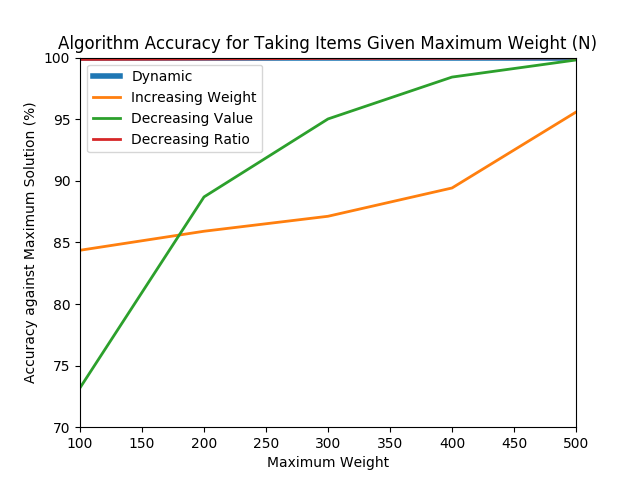
\includegraphics[width=0.70\textwidth]{python/accuracyGraph.png}
			\caption{Algorithm Accuracy for Taking Items Given Maximum Weight $n$}
			\label{fig:accuracy-graph}
		\end{center}
	\end{figure}
	% Diagram showing the % accuracy of different approaches
	\begin{figure}[htbp]
		\begin{center}
			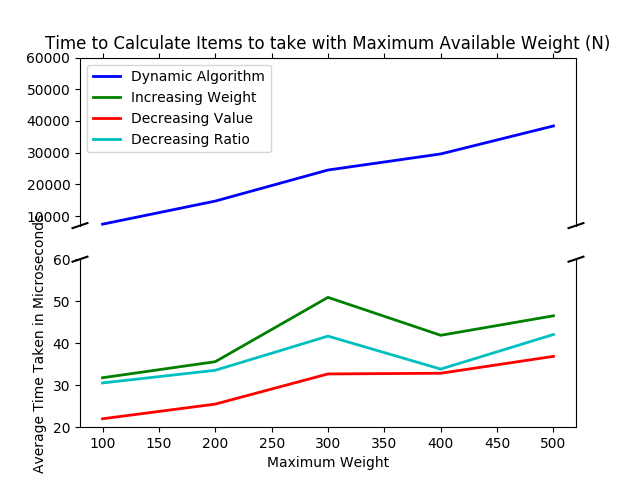
\includegraphics[width=0.70\textwidth]{python/timeGraph.png}
			\caption{Time to Calculate Items to take with Maximum Available Weight $n$}
			\label{fig:time-graph}
		\end{center}
	\end{figure}
\section{Conclusions}

\end{document}
